\documentclass{article}
\usepackage{svg}
\usepackage{caption}
\usepackage{subcaption}
\usepackage{graphicx}
\usepackage{tabularx}

\usepackage[margin=1in]{geometry} % for 1 inch side panels


\begin{document}

\begin{titlepage}
    \centering
    \vspace*{0cm}
    {\scshape\Large Frankfurt University of Applied Sciences}\\[3cm]
    {\huge\bfseries Title}\\[8cm]
    {\Large\itshape Group 6:}\\
    {\Large\itshape Hermon Giikael, Howard-Yi Hong Soon, Jiwon Won, Lars Friese, Marc Roemer, Stefan Nguyen}\\[4cm]
    Supervisor:\\
    Jörg Schäfer\\[3cm]
    {\large \today}
\end{titlepage}

\tableofcontents
\newpage

\section{Hermon Gimikael}

	\subsection{Requirement1}
		\begin{figure}[h!]
		    \centering
		    \captionsetup{labelformat=empty}
		    \caption{Your caption}
		    \includegraphics[width=\textwidth, angle=0]{Kreis2.pdf}
		\end{figure}
		\newpage
		\begin{figure}[h!]
		    \centering
		    \captionsetup{labelformat=empty}
		    \caption{Your caption}
		    \includegraphics[width=\textwidth, angle=0]{Kreis2.pdf}
		\end{figure}
		\newpage
	
	\subsection{Requirement2}
		\begin{figure}[h!]
		    \centering
		    \captionsetup{labelformat=empty}
		    \caption{Your caption}
		    \includegraphics[width=\textwidth, angle=0]{Kreis2.pdf}
		\end{figure}
		\newpage

\section{Howard-Yi Hong Soon}
		\subsection{Requirement 10: Easy usability with Gesture Control}
		\begin{center}
			\begin{tabularx}{1.0\textwidth}{|>{\raggedright\arraybackslash}p{0.2\textwidth}|>{\raggedright\arraybackslash}X|}
				\hline
				Name             & Share workout achievements on social media \\ \hline
				ID               & 5 \\ \hline
				Business Value   & Low \\ \hline
				Description      & Create workout achievements page and share it to logged-in social media \\ \hline
				Trigger          & Push "share" button and chose specific social media to be delivered achievement page\\ \hline
				Actors           & User, Workout System, Social Media System\\ \hline
				Pre-conditions   & User successfully logged in social media, internet connected\\ \hline
				Post-conditions  & User post workout achievement page on social media\\ \hline
				Basic Flow       & \\ \hline
								Description Actions& This is the main scenario when user has an achievement to share and linked social media account \\ \hline
								1 & The use chooses an achievement to share \\ \hline
								2 & The workout system creates the achievement post \\ \hline
								3 & The user chooses a social media app to share \\ \hline
								4 & The workout system sends the achievement post to the social media system \\ \hline
				Alternative Flow & A \\ \hline
								Description Actions& There isn't any achievement to share \\ \hline
								1 & The workout system shows "Start workout and share it" \\ \hline
				Alternative Flow & B \\ \hline
								Description Actions& The searched item is not found in the database and shows an error \\ \hline
								1 & The app requests the user to manually input the nutritional information's about the item \\ \hline
								2 & User has to tip in calories, nutrients, serving size and name of the item and saves it \\ \hline
								3 & The app takes the data through a verification process and adds it to the food database \\ \hline
			\end{tabularx}
		\end{center}
	\newpage

	\begin{figure}[htbp]
		\centering
		\begin{subfigure}{\textwidth}
			\resizebox{\textwidth}{!}{\includesvg[]{Howard/share_workout/ShareWorkoutAchievement_usecase.svg}}
			\caption{Use Case Diagram}
		\end{subfigure}
		\begin{subfigure}{\textwidth}
			This ShareWorkoutAchievement use case shows the operations and the interaction between system and user
			of the requirement. It has a few of includes and extends, e.g. display message "start workout and share it" and
			select achievement, the user has to click on share button in order to trigger them. "Share achievement on Social Media" has an extend
			optional function to download image. 
		\end{subfigure}
	\end{figure}
	\newpage

	\begin{figure}[htbp]
		\centering
		\begin{subfigure}{\textwidth}
			\resizebox{\textwidth}{!}{\includesvg[]{Howard/share_workout/ShareWorkoutAchievement_usecase.svg}}
			\caption{Use Case Diagram}
		\end{subfigure}
		\begin{subfigure}{\textwidth}
			This ShareWorkoutAchievement use case shows the operations and the interaction between system and user
			of the requirement. It has a few of includes and extends, e.g. display message "start workout and share it" and
			select achievement, the user has to click on share button in order to trigger them. "Share achievement on Social Media" has an extend
			optional function to download image. 
		\end{subfigure}
	\end{figure}
	\newpage

	\begin{figure}[htbp]
		\centering
		\begin{subfigure}{\textwidth}
			\resizebox{\textwidth}{!}{\includesvg[]{Howard/share_workout/ShareWorkoutAchievement_activity.svg}}
			\caption{Use Case Diagram}
		\end{subfigure}
		\begin{subfigure}{\textwidth}
			This ShareWorkoutAchievement use case shows the operations and the interaction between system and user
			of the requirement. It has a few of includes and extends, e.g. display message "start workout and share it" and
			select achievement, the user has to click on share button in order to trigger them. "Share achievement on Social Media" has an extend
			optional function to download image. 
		\end{subfigure}
	\end{figure}
	\newpage

\section{Jiwon Won}
	\subsection{Requirement1}
		\begin{figure}[h!]
		    \centering
		    \captionsetup{labelformat=empty}
		    \caption{Your caption}
		    \includegraphics[width=\textwidth, angle=0]{Kreis2.pdf}
		\end{figure}
		\newpage
		\begin{figure}[h!]
		    \centering
		    \captionsetup{labelformat=empty}
		    \caption{Your caption}
		    \includegraphics[width=\textwidth, angle=0]{Kreis2.pdf}
		\end{figure}
		\newpage



\section[]{Lars Friese}
	\subsection{Requirement 10: Easy usability with Gesture Control}
	\begin{center}
		\begin{tabularx}{1.0\textwidth}{|>{\raggedright\arraybackslash}p{0.2\textwidth}|>{\raggedright\arraybackslash}X|}
			\hline
			Name             & Use gestures to execute actions on smartwatch \\ \hline
			ID               & 12 \\ \hline
			Business Value   & medium \\ \hline
			Description      & When the user lifts his arm and turns his wrist the smartwatch display turns on, when he lowers the arm the display turns of. Additionally the smartwatch executes a costum gesture \\ \hline
			Trigger          & User lifting/lowering arm and turning wrist or shaking his wrist \\ \hline
			Actors           & User, System, Gyroscope Sensor\\ \hline
			Pre-conditions   & Display is turned on/off\\ \hline
			Post-conditions  & Display is turned on/off, App opened\\ \hline
			Basic Flow       & \\ \hline
							  Description & This is the main scenario where the system recognizes the hand up movement \\ \hline
							  Actions & \\ \hline
							  1 & User raises arm \\ \hline
							  2 & System recognizes gesture \\ \hline
							  3 & Display turns on \\ \hline
			Alternative Flow & A \\ \hline
							  Description & Actions \\ \hline
							  & 1 \\ \hline
							  & 2 \\ \hline
			Alternative Flow & B \\ \hline
							  Description & Actions \\ \hline
							  & 1 \\ \hline
							  & 2 \\ \hline
							  & 3 \\ \hline
							  & 4 \\ \hline
							  & 5 \\ \hline
		\end{tabularx}
	\end{center}

	\begin{figure}[htbp]
		\centering
		\begin{subfigure}{\textwidth}
			\resizebox{\textwidth}{!}{\includesvg[]{Lars/Use Case Gesture Control/GestureControl_usecase.svg}}
			\caption{Use Case Diagram}
		\end{subfigure}
		\begin{subfigure}{\textwidth}
			Example text 1 \
			Example text 2
		\end{subfigure}
	\end{figure}
	
	\begin{figure}[htbp]
		\centering
		\begin{subfigure}{\textwidth}
			\resizebox{\textwidth}{!}{\includesvg[]{Lars/Use Case Gesture Control/GestureControl_activity.svg}}
			\caption{Activity Diagram}
		\end{subfigure}
		\begin{subfigure}{\textwidth}
			Example text 3 \\
			Example text STARWBERRY 
		\end{subfigure}
	\end{figure}
	
	\begin{figure}[htbp]
		\centering
		\begin{subfigure}{\textwidth}
			\resizebox{\textwidth}{!}{\includesvg[]{Lars/Use Case Gesture Control/GestureControl_class.svg}}
			\caption{Class Diagram}
		\end{subfigure}
		\begin{subfigure}{\textwidth}
			Example text 5 \\
			Example text 6 
		\end{subfigure}
	\end{figure}
	
	\begin{figure}[htbp]
		\centering
		\begin{subfigure}{\textwidth}
			\resizebox{\textwidth}{!}{\includesvg[]{Lars/Use Case Gesture Control/GestureControl_sequence.svg}}
			\caption{Sequence Diagram}
		\end{subfigure}
		\begin{subfigure}{\textwidth}
			Example text 7 \\
			Example text 8
		\end{subfigure}
	\end{figure}
\newpage


\section{Marc Roemer}
	\subsection{Requirement 9: Calculation and display daily and weekly step count statistics}
		\begin{figure}[h!]
			\centering
			\captionsetup{labelformat=empty}
			\caption{UseCase}
		\end{figure}
		\newpage
		\begin{figure}[h!]
			\centering
			\captionsetup{labelformat=empty}
			\caption{UI Prototype}
		\end{figure}
		\newpage
		\begin{figure}[h!]
		    \centering
		    \captionsetup{labelformat=empty}
		    \caption{Activity Diagram}
		    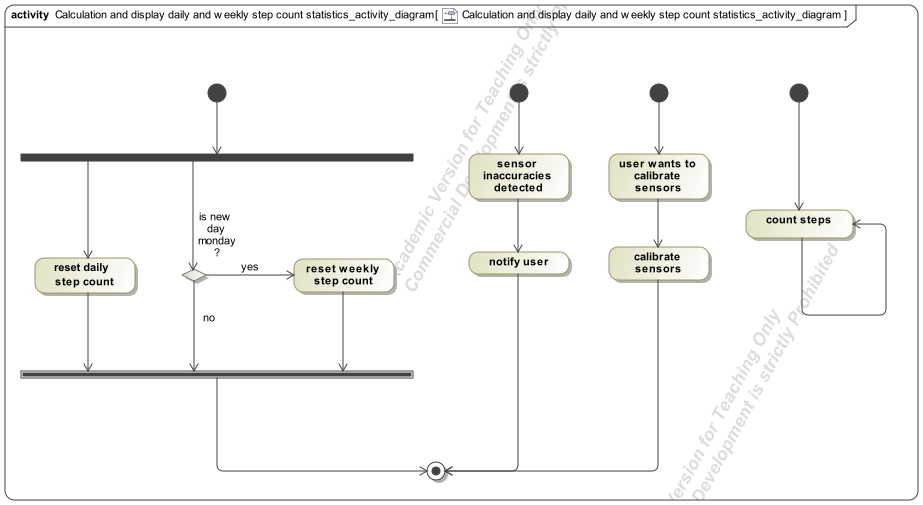
\includegraphics[width=\textwidth, angle=0]{Marc/req9/9activity.pdf}
		\end{figure}
		\newpage
		\begin{figure}[h!]
			\centering
			\captionsetup{labelformat=empty}
			\caption{UseCase Diagram}
		\end{figure}
		\newpage
		\begin{figure}[h!]
			\centering
			\captionsetup{labelformat=empty}
			\caption{Sequence Diagram}
		\end{figure}
		\newpage
		\begin{figure}[h!]
			\centering
			\captionsetup{labelformat=empty}
			\caption{Class Diagram}
		\end{figure}
		\newpage

	\subsection{Requirement 10: Create and manages a workout plan}
		\begin{figure}[h!]
			\centering
			\captionsetup{labelformat=empty}
			\caption{UseCase}
		\end{figure}
		\newpage
		\begin{figure}[h!]
			\centering
			\captionsetup{labelformat=empty}
			\caption{UI Prototype}
		\end{figure}
		\newpage
		\begin{figure}[h!]
		    \centering
		    \captionsetup{labelformat=empty}
		    \caption{Activity Diagram}
		    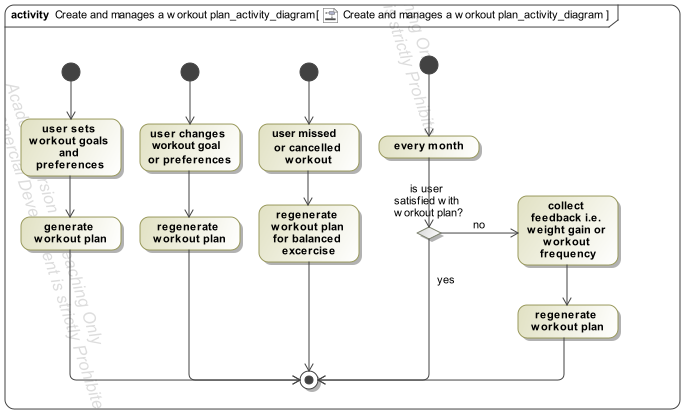
\includegraphics[width=\textwidth, angle=0]{Marc/req10/10activity.pdf}
		\end{figure}
		\newpage
		\begin{figure}[h!]
			\centering
			\captionsetup{labelformat=empty}
			\caption{UseCase Diagram}
		\end{figure}
		\newpage
		\begin{figure}[h!]
			\centering
			\captionsetup{labelformat=empty}
			\caption{Sequence Diagram}
		\end{figure}
		\newpage
		\begin{figure}[h!]
			\centering
			\captionsetup{labelformat=empty}
			\caption{Class Diagram}
		\end{figure}
		\newpage
			

\section{Stefan Nguyen}
	\subsection{Display Heart Rate Data on Smartwatch}
	\begin{center}
		\begin{tabularx}{1.0\textwidth}{|>{\raggedright\arraybackslash}p{0.2\textwidth}|>{\raggedright\arraybackslash}X|}
			\hline
			Name             & Environment monitoring \\ \hline
			ID               & 11 \\ \hline
			Business Value   & Low \\ \hline
			Description      & Tracks UV exposure, air quality, temperature in real time \\ \hline
			Trigger          & Typical event which adjusts the changes in real time \\ \hline
			Actors           & Environmental Sensor Array, which is responsible for capturing environmental data \\ \hline
			Pre-conditions   & Environmental sensors are operational and calibrated\\ \hline
			Post-conditions  & Displays the data in the smartwatch\\ \hline
			Basic Flow       & \\ \hline
							  Description & Detail each change in the environment monioring system \\ \hline
							  Actions & \\ \hline
							  1 & activating the sensors \\ \hline
							  2 & capturing the data (e.g. temperature, UV, etc) \\ \hline
							  3 & processing data e.g. analysis or computations \\ \hline
							  4 & transfer data into smartwatch \\ \hline
							  5 & display data in smartwatch \\ \hline
			Alternative Flow & A \\ \hline
							  Description & Error capturing data (network, communication etc) \\ \hline
							  1 & sensor fails to capture data \\ \hline
							  2 & fail, communication or network error in smartwatch or sensor \\ \hline
							  3 & Error capturing data / false data display information \\ \hline
			Alternative Flow & B \\ \hline
							  Description & Environmental sensor detect conditions which my threaten health conditions \\ \hline
							  1 & sensor detects hazardous condition and flag it as highest priority \\ \hline
							  2 & sends push notification and warns the user \\ \hline
							  3 & displays the notification on the smartwatch and recommends actions (e.g. apply sunscreen, seek shelter, etc) \\ \hline
							  4 & user acknowledges the notification\\ \hline
							  5 & user doesn't acknoweldege notification -> the system keeps sending notifications or warns the user \\ \hline
		\end{tabularx}
	\end{center}
	\newpage

	\begin{figure}[htbp]
		\centering
		\begin{subfigure}{\textwidth}
			\resizebox{\textwidth}{!}{\includesvg[]{Stefan/Environment Monitoring/EnvironmentMonitoring_use_case_diagram.svg}}
			\caption{Use Case Diagram}
		\end{subfigure}
		\begin{subfigure}{\textwidth}
			The Environment Monitoring shows the use cases. The Actvity sensor sensors the environment and transmit
			proceeds the data and generate a safe monioring notification. This tells the user the current environement e.g.
			temperature, UV exposure or more. If it comes to hazardous conditions it sends the user a notification and asks him 
			to either acknoweldege or not. Next the activity sensor displays the data on the smartwatch and record or
			track any other incident reports. The user on the other hand can acknoweldege the notification and look into
			history data and has an authentification. 
		\end{subfigure}
	\end{figure}
	\newpage

	\begin{figure}[htbp]
		\centering
		\begin{subfigure}{\textwidth}
			\resizebox{\textwidth}{!}{\includesvg[]{Stefan/Environment Monitoring/EnvironmentMonitoring_activity_diagram.svg}}
			\caption{Activity Diagram}
		\end{subfigure}
		\begin{subfigure}{\textwidth}
			The activity diagram shows a walkthrough of the operations or activities that need to be done, 
			so it can monitor the environment. Firstly, it activates the sensor and collects all the environment 
			data and transmits/proceeds them. It later asks for safe monitoring to ensure that there are no incidents 
			like hazards or natural disasters. If the user clicks no then the system prepares the notification and 
			asks the user to acknowledge the alert. The alert shows tips or recommendations which need to be done, to 
			shorten the risk of endangering personal life. If the user doesn’t accept the notification then the system 
			keeps warning the user or keeps spamming alerts, else it displays the data with the notification.
		\end{subfigure}
	\end{figure}
	\newpage

	\begin{figure}[htbp]
		\centering
		\begin{subfigure}{\textwidth}
			\resizebox{\textwidth}{!}{\includesvg[]{Stefan/Environment Monitoring/EnvironmentMonitoring_class_diagram.svg}}
			\caption{Class Diagram}
		\end{subfigure}
		\begin{subfigure}{\textwidth}
			The UML shows the structure of the classes, how they interact with each other and what methods are 
			used later in the sequence diagram. For example, the Activity Sensor sends data to the process data 
			which is a unidirectional relation with 1. The activity sensor has methods like activate sensor, keep 
			monitoring and stop monitoring. The monitoring would work permanently while the smartwatch is on. The 
			process list has the notifications, hazardous condition and process data and uses the unidirectional 
			relation to the display. While the display formats the data to the smartwatch so that the user can access 
			the data and can see the outputted data. 
		\end{subfigure}
	\end{figure}
	\newpage

	\begin{figure}[htbp]
		\centering
		\begin{subfigure}{\textwidth}
			\resizebox{\textwidth}{!}{\includesvg[]{Stefan/Environment Monitoring/EnvironmentMonitoring_sequence_diagram.svg}}
			\caption{Sequence Diagram}
		\end{subfigure}
		\begin{subfigure}{\textwidth}
			The sensor diagram almost works the same way as the display heartbeat data. It activates the sensor, 
			does the process and checks for hazardous conditions in the environment and does the following alternative
			operations. Later it either sends a notification or outputs the data to the display of the smartwatch. 
			The small part of smartwatch on represents that the sensor works permanently and keeps monitoring until 
			the smartwatch is off. 
		\end{subfigure}
	\end{figure}
	\newpage

\end{document}